\documentclass[11pt]{ctexart}

\usepackage{multicol}
%\usepackage{mwe}
\usepackage{subfigure}
\usepackage{mathtools}
\usepackage{graphicx}
\usepackage{amsmath}
\usepackage{mathrsfs}
\usepackage[top=0.5in,bottom=1in,left=1in,right=1in]{geometry}
\usepackage{pdflscape}
\usepackage{times}
\usepackage{bm}
%\usepackage{setspace}
\usepackage{color}
\usepackage{caption}
\usepackage{amsmath}
\usepackage{amssymb}
\usepackage{CJK}
\usepackage{longtable}
%\usepackage[final]{pdfpages}
\usepackage{listings}
\usepackage{textcomp}
\usepackage{xcolor}
\usepackage{algorithm2e}
\usepackage{float}
\usepackage{algorithmicx}
\usepackage{algpseudocode}
\usepackage{hyperref}

\hypersetup{hidelinks,
	colorlinks=true,
	allcolors=black,
	pdfstartview=Fit,
	breaklinks=true}

\pagestyle{plain}




\begin{document}

\title{第七周实习报告20220426}
\author{宋欣源}
\date{\today}

\maketitle % need full-width title

\CTEXsetup[format={\Large\bfseries}]{section}

\section{第一,综述}

下面对于这些天实习的工作做一个报告。现在就两周的工作做一个总结
我这周主要分成三个大的方向,1.模型的再修正,2.convolutedRNNcell,3.基于transformer的BERT和GPT的 baseline模型以及思考。

\section{第二,模型的再修正}

\subsection{1.对于神经网络和参数的梳理和归纳}
首先对于神经网络的基础和参数进行了重修,掌握了很多缺漏和补充知识。

\subsubsection{Convolution}
Conv1d
\begin{itemize}
  \item [1)]
  in\_channels 输入的维度
  \item [2)]
  out\_channels 输出的维度
  \item [3)]
  kernel\_size 卷积核的大小
  \item [4)]
  stride 每次卷积卷积核在seqlength(S)上移动的步幅,默认为1,可以处理分别卷积和滑动卷积
  \item [5)]
  padding 默认为0,代表卷积两侧因为卷积核而使序列在seqlength(S)上尺寸缩短的部分
  \item [6)]
  dilation代表膨胀卷积,是卷积核并非均匀的从目标上采样,而是每个采样点在seqlength(S)上有一个步幅。因此,对于kernel\_size, padding,dilation,stride,和输出输出序列长度的关系,有
\end{itemize}

$$L_{out} = \left[ \frac{L_{in} + 2 \cdot padding - dilation \cdot (kernel\_size -1) -1}{stride} + 1 \right]$$

\begin{itemize}
  \item [7)]
  groups 控制输入和输出维度(F)的相互关系,in\_channels和out\_channels都要被groups整除。\par $groups=1$表示整个是一个组,每个卷积核的维度是$(kernel\_size, in\_channels, out\_channels)$,在计算时,先对每个in\_channels的卷积核上做卷积,再把这些卷积结果加起来,\par 合并成kernel\_size的维度,剩下out\_channels就是输出维度。例如,$groups = 2$,就是将in\_channels分成两部分,分别输出到out\_channels的两部分。$groups = in\_channels$代表每个输入都自己是一个组,灭个卷积核只作用到自己的维度。
  \item [2)]
  bias 卷积所携带的常数参数
  \item [3)]
  padding\_mode padding的方式,有如下几种: zeros代表用0来padding,replicate代表用最外侧的数字来补全,reflect代表用最外层内部的数值反射填充到最外层,circular代表用矩阵自己来填充自己,所以对应用最下层填充最上层的padding位置。目前来看应该采用replicate最合适,及不会影响原本数字意义,又不会影响时间序列的效果。在pooling的时候填充模式还有更好的算法,在后面介绍。
  \item [4)]
  device 卷积核所在的设备名称:cuda
  \item [5)]
  dtype 卷积核的数据类型
\end{itemize}


卷积的计算方法:公式
$$out(N_i, C_{out_j}) = bias(C_{out_j}) + \Sigma^{C_{in}-1}_{k=0} weight(C_{out_j}, k) * input(N_i,k)$$

计算方法:将卷积核和要卷积的部分展平。利用nn.Fold来实现,然后对每个卷积核作用的地方和卷积核展成的一维张量,计算点积。这就是单次卷积的实现。然后将卷积核的输入维度全部相加。输出到输出维度,再用nn.unFold将一维张量点积变成目标平面。

信息流:从输入上先乘以卷积核中的参数,到达卷积核。相当于使卷积核获得了他的感受野范围内的一个整体观点。再用多个卷积核相加,共同表达这一片区域。信息就经过过滤和提取到达新的卷积层。由于在运算过程中,卷积会使得边界越来越清晰(原来较大的数字越来越大,较小的数字越来越小)所以就相当于把边界信息储存在卷积核之中。这些边界信息经过全连接层和展平层,可以当作输出的分类信号。

unfold: 这个操作将每一个kernel\_size的数据方块展平成一个新的维度,同时剩下L的维度,\par $(N,C,s) \rightarrow (N,C, \prod (kernel\_size),L)$,用这个方法,将$(N,C,C_{out},\prod (kernel\_size))$的卷积核同样进行展平。二者相乘后数据变成$(N,C_{out}, \prod (kernel\_size),L)$,然后再用nn.fold也就是unfold的逆运算变成结果的样子。同时,fold和unfold还兼顾dilation,padding和stride的结构,有:
$$L_{out} = \prod_d \left[ \frac{spatial\_size[d] + 2 \cdot padding[d] - dilation[d] \cdot (kernel\_size[d] -1) -1}{stride[d]} + 1 \right]$$

~\\
Conv2d和Conv1d的做法完全一样,只是卷积操作的维度从一维变成两维,卷积核的维度从一维(1*3)变成两维(3*3)

\subsubsection{pooling}
MaxPool1d
\begin{itemize}
  \item [1)]
  kernel\_size 计算最大值区域的大小
  \item [2)]
  stride 每次计算最大值的区域核在seqlength(S)上移动的步幅,默认为kernel\_size,改成1可以计算滑动max。
  \item [3)]
  padding 默认为0,代表在原来序列在seqlength(S)上两端添加的数值0
  \item [4)]
  dilation代表膨胀计算,是核并非均匀的从目标上采样,而是每个采样点在seqlength(S)上有一个步幅。因此,对于kernel\_size, padding,dilation,stride,和输出输出序列长度的关系,有
\end{itemize}

$$L_{out} = \left[ \frac{L_{in} + 2 \cdot padding - dilation \cdot (kernel\_size -1) -1}{stride} + 1 \right]$$

\begin{itemize}
  \item [5)]
  return\_indices 是否返回最大值所在的位置,使用maxpool的结果构造稀疏矩阵的时候(layout= sparse\_coo)将indices和values都传入下一层参数。
  \item [6)]
  ceil\_mode 如果最大值的结果区域大小为小数,是否向上取整(填补0),由于max的填补0不会影响最后结果,所以填补方式不影响结果。

\end{itemize}

~\\
Maxpool2d和Maxpool3d和一维情况几乎一样,不专门写。

AvgPool1d
\begin{itemize}
  \item [1)]
  kernel\_size 计算平均值区域的大小
  \item [2)]
  stride 每次计算平均值的区域核在seqlength(S)上移动的步幅,默认为kernel\_size,改成1可以计算滑动max。
  \item [3)]
  padding 默认为0,代表在原来序列在seqlength(S)上两端添加的数值0

\end{itemize}

$$L_{out} = \left[ \frac{L_{in} + 2 \cdot padding -  kernel\_size -1}{stride} + 1 \right]$$

\begin{itemize}
  \item [4)]
  ceil\_mode 如果最大值的结果区域大小为小数,是否向上取整(填补0),由于mean的填补0对结果影响很大,所以有新的参数。
  count\_include\_pad 表示padding的0不计算进入mean。这个参数很重要,一定设置为True

\end{itemize}

~\\
Avgpool2d和Avgpool3d和一维情况不太一样,当在区域上取平均或者在立方体上取平均的时候,默认是除以kernel\_size的,或者可以自己设置divisor\_override参数,自定义除数大小。

\subsubsection{Linear}
Linear
计算线性层$y = x A^T + b$
\begin{itemize}
  \item [1)]
  in\_features 输入的通道数
  \item [2)]
  in\_features 输出的通道数
  \item [3)]
  bias 是否加常数项b
  \item [4)]
  device: cuda
  \item [5)]
  dtype: 数据类型
\end{itemize}

\subsubsection{Embedding}
Embedding
embedding的作用在下面会用到。作用是将seq数据转换成线性张量组。embedding\_dim视为语义张量的维度,\par 在本任务中,把close, volume, turnover看成语义的三个维度,时间维度看成语句,相似的语义一般看成线性相关程度大的向量。因此在下面运用baseline model的时候,其实是把embedding层放入BERT进行训练。
\begin{itemize}
  \item [1)]
  num\_embeddings 字典的大小,这个参数没用。一般embeddings的参数需要预训练好。
  \item [2)]
  embedding\_dim seq模型的通道数

\end{itemize}

\subsubsection{RNN}
nn.RNN
RNN计算公式如下$h_t = tanh(W_{ih} x_t +b_{ih} +W_{hh}h_{(t-1)} +b_{hh})$,将每一个输入x输入到RNNcell里,经过这个线性层的计算,输出h\_state和c\_state,在RNNbase里将新的h\_state和c\_state和下一时刻的输入带入RNNcell.
\begin{itemize}
  \item [1)]
  input\_size 输入的通道数
  \item [2)]
  hidden\_size 隐藏层的维度
  \item [3)]
  num\_layers rnnbase里的cell的个数,每层是一个新的cell
  \item [4)]
  nonlinearity 非线性激活函数
  \item [5)]
  batch\_first 指的是batch是在于第一个还是第二个,一般rnn都要求seqlength在第一个,\par 如果batch\_first为True的话batch在第一个
  \item [6)]
  dropout 丢失层
  \item [7)]
  bidirectional 如果True那么顺序进行一侧RNN外还会从最后一分钟开始反向进行一次RNNcell

\end{itemize}

nn.LSTM和nn.GRU算法相同
LSTM的公式如下:
\begin{equation}
\begin{split}
    i_t &= \sigma (W_{x i} x_t + W_{H i} h_{t-1} + b_i)\\
    f_t &= \sigma (W_{x f} x_t + W_{H f} h_{t-1} + b_f)\\
    c_t &= f_t \odot c_{t-1} + i_t \odot \tanh (W_{x c} x_t + W_{H c} h_{t-1} + c_i)\\
    o_t &= \sigma (W_{x o} x_t + W_{H o} h_{t-1} + b_o)\\
    h_t &= o_t \odot \tanh(c_t)
\end{split}
\end{equation}

GRU的公式如下:
\begin{equation}
\begin{split}
    f_t &= \sigma (W_{x_t f} +W_{H f} h_{t-1} + b_f)\\
    c_t &= f_t \odot c_{t-1} + (1-f_t) \odot \tanh (W_{x_t c} x_t +W_{H c} h_{t-1} + b_c)\\
    o_t &= \sigma (W_{x_t o} x_t +W_{H o} h_{t-1} + b_o)\\
    h_t &= o_t \odot \tanh(c_t)
\end{split}
\end{equation}

将每一个输入x输入到RNNcell里,经过这个线性层的计算,输出h\_state和c\_state,在RNNbase里将新的h\_state和c\_state和下一时刻的输入带入RNNcell.LSTM和GRU的多个门可以通过一个大的线性层进行计算,\par 可以大大减少计算时间。

\subsubsection{修正后模型的效果和分析}
按照上述方式对原有模型进行改进,避免的尺度减少,同时照顾了边界计算问题,使得模型性能有小幅提高。

模型1:普通CNN2d(ordinary*2+pointwise+linear*2+dropout+relu)

{\kaishu \small IC: 0.058, pnl:2.0}

原有模型:
{\kaishu \small IC\_old: 0.056, pnl\_old:1.9}

~\\
模型2:普通CNN2d(deepwise*2+pointwise+linear*2+dropout+relu)

{\kaishu \small IC: 0.057, pnl:2.1}

原有模型:
{\kaishu \small IC\_old: 0.056, pnl\_old:1.9}

~\\
模型3:普通CNN2d(ordinary*2+linear*2+pointwise+linear*2+dropout+relu)

{\kaishu \small IC: 0.048, pnl:1.9}

原有模型:
{\kaishu \small IC\_old: 0.046, pnl\_old:1.9}

~\\
模型4:普通CNN2d(deepwise*2+linear*2+pointwise+linear*2+dropout+relu)

{\kaishu \small IC: 0.062, pnl:2.0}

原有模型:
{\kaishu \small IC\_old: 0.056, pnl\_old:1.9}

~\\
模型5:普通CNN2d(deepwise*2+maxpool+linear*2+pointwise+linear*2+dropout+relu)

{\kaishu \small IC: 0.042, pnl:1.8}

原有模型:
{\kaishu \small IC\_old: 0.041, pnl\_old:1.7}

~\\
模型6:普通CNN2d(deepwise*2+ordinary+linear*2+pointwise+linear*2+dropout+relu)

{\kaishu \small IC: 0.066, pnl:2.2}

原有模型:
{\kaishu \small IC\_old: 0.065, pnl\_old:2.1}

~\\
模型7:普通CNN2d(deepwise*2+ordinary*3+linear*2+pointwise+linear*2+dropout+relu)

{\kaishu \small IC: 0.068, pnl:2.4}

原有模型:
{\kaishu \small IC\_old: 0.065, pnl\_old:2.1}

~\\
CNN1d的应用范围就非常广了,可以将时间序列当成一维音频数据,进行提取,也不用考虑过多的技巧。因此在一维CNN上设计了大量模型进行尝试。

模型8:普通CNN1d(ordinary*2+avg+linear*2+dropout+relu)

{\kaishu \small IC: 0.042, pnl:1.8}

原有模型:
{\kaishu \small IC\_old: 0.044, pnl\_old:1.9}

~\\
模型9:普通CNN1d(ordinary*2+avg+ordinary*2+linear*2+dropout+relu)

{\kaishu \small IC: 0.045, pnl:1.9}

原有模型:
{\kaishu \small IC\_old: 0.045, pnl\_old:2.0}

~\\
模型10:普通CNN1d(ordinary*2+avg+ordinary*2+linear*2+pointwise+dropout+relu)

{\kaishu \small IC: 0.052, pnl:1.9}

原有模型:
{\kaishu \small IC\_old: 0.045, pnl\_old:1.8}

~\\
模型11:普通CNN1d((ordinary+avg+relu)*3+(ordinary+relu)*2+ordinary+linear*2+dropout+relu)

{\kaishu \small IC: 0.052, pnl:1.8}

原有模型:
{\kaishu \small IC\_old: 0.053, pnl\_old:2.0}

~\\
模型12:普通CNN1d((ordinary+avg+relu)*3+(ordinary+relu)*3+ordinary+linear*2+dropout+relu)

{\kaishu \small IC: 0.050, pnl:2.0}

原有模型:
{\kaishu \small IC\_old: 0.049, pnl\_old:2.0}

~\\
模型13:普通CNN1d((ordinary+avg+relu)*4+(ordinary+relu)*3+ordinary+linear*2+dropout+relu)

{\kaishu \small IC: 0.050, pnl:2.1}

原有模型:
{\kaishu \small IC\_old: 0.049, pnl\_old:2.0}

~\\
模型14:普通CNN1d((ordinary+avg+relu)*5+(ordinary+relu)*3+ordinary+linear*2+dropout+relu)

{\kaishu \small IC: 0.061, pnl:2.25}

原有模型:
{\kaishu \small IC\_old: 0.056, pnl\_old:2.1}

~\\
模型15:普通CNN1d((ordinary+avg+relu)*6+(ordinary+relu)*3+ordinary+linear*2+dropout+relu)

{\kaishu \small IC: 0.070, pnl:2.42}

原有模型:
{\kaishu \small IC\_old: 0.056, pnl\_old:2.1}

~\\
模型16:bottleneck((cnn1d(1)+cnn1d(3)+cnn1d(1))+pointwise+linear+dropout+relu)

{\kaishu \small IC: 0.060, pnl:1.7}

原有模型:
{\kaishu \small IC\_old: 0.058, pnl\_old:1.8}

~\\
模型17:bottleneck((cnn1d(1)+cnn1d(3)+cnn1d(1))+pointwise+linear+dropout+relu)


{\kaishu \small IC: 0.059, pnl:1.7}

原有模型:
{\kaishu \small IC\_old: 0.061, pnl\_old:1.9}

~\\
模型18:base((cnn1d+batchnorm+relu+avgpool)*2+pointwise+linear+dropout+relu)

{\kaishu \small IC: 0.031, pnl:1.4}

原有模型:
{\kaishu \small IC\_old: 0.031, pnl\_old:1.4}

~\\
模型19: bottleneck((cnn1d+batchnorm+relu+avgpool)*2+bottleneck1+pointwise

+linear+dropout+relu)

{\kaishu \small IC: 0.035, pnl:1.5}

原有模型:
{\kaishu \small IC\_old: 0.045, pnl\_old:1.8}

~\\
模型20: bottleneck((cnn1d+batchnorm+relu+avgpool)*2+bottleneck2+pointwise

+linear+dropout+relu)

{\kaishu \small IC: 0.039, pnl:1.37}

原有模型:
{\kaishu \small IC\_old: 0.046, pnl\_old:1.6}

可以看出,在模型18和19上序列缩短效果较好。

~\\
模型21: bottleneck((cnn1d+batchnorm+relu+avgpool)*2+bottleneck1+bottleneck2+pointwise

+linear+dropout+relu)

{\kaishu \small IC: 0.045, pnl:1.4}

原有模型:
{\kaishu \small IC\_old: 0.048, pnl\_old:1.9}

从模型21开始恢复正常,修正模型的效果稍微强一点。

~\\
模型22: deepnn((cnn1d+batchnorm+relu+avgpool)*2+bottleneck1

+bottleneck2+bottleneck1+bottleneck2+pointwise+linear+dropout+relu)

{\kaishu \small IC: 0.068, pnl:2.0}

原有模型:
{\kaishu \small IC\_old: 0.065, pnl\_old:2.1}

~\\
模型23: multigrid(base+multigrid+poitwise)

{\kaishu \small IC: 0.073, pnl:2.3}

原有模型:
{\kaishu \small IC\_old: 0.069, pnl\_old:2.2}

当模型复杂的时候,序列越长模型表现越不稳定,短序列的优点是模型稳定,长序列则表现不太稳定,往往需要多次run才能得到理想的结果。

~\\
模型24: multigrid+bottleneck(base+bottleneck+multigrid\_assp+linear)

{\kaishu \small IC: 0.071, pnl:2.3}

原有模型:
{\kaishu \small IC\_old: 0.065, pnl\_old:2.1}

~\\
模型25:multigrid+bottleneck(base+bottleneck+multigrid\_batchnorm+linear)

{\kaishu \small IC: 0.072, pnl:2.3}

原有模型:
{\kaishu \small IC\_old: 0.065, pnl\_old:2.1}

~\\26:multigrid+bottleneck(base+bottleneck+multigrid\_batchnorm+linear)

计算出的结果还是一样。

{\kaishu \small IC: 0.072, pnl:2.3}

原有模型:
{\kaishu \small IC\_old: 0.071, pnl\_old:2.4}

~\\
模型27:multigrid+bottleneck(base+bottleneck+multigrid\_batchnorm+linear)

{\kaishu \small IC: 0.068, pnl:2.1}

原有模型:
{\kaishu \small IC\_old: 0.065, pnl\_old:2.1}

~\\
模型28:multigrid+bottleneck(base+bottleneck+multigrid\_batchnorm+downsample)

{\kaishu \small IC: 0.064, pnl:2.1}

原有模型:
{\kaishu \small IC\_old: 0.064, pnl\_old:2.1}

~\\
模型29:multigrid(multigrid\_batchnorm+downsample)

{\kaishu \small IC: 0.070, pnl:2.45}

原有模型:
{\kaishu \small IC\_old: 0.071, pnl\_old:2.2}

~\\
模型30:multigrid(multigrid\_batchnorm+downsample+upsample)

{\kaishu \small IC: 0.070, pnl:2.3}

原有模型:
{\kaishu \small IC\_old: 0.065, pnl\_old:2.1}

~\\
模型31:multigrid(multigrid\_batchnorm+downsample+upsample)

{\kaishu \small IC: 0.078, pnl:2.45}

\begin{figure}[H]
\begin{center}
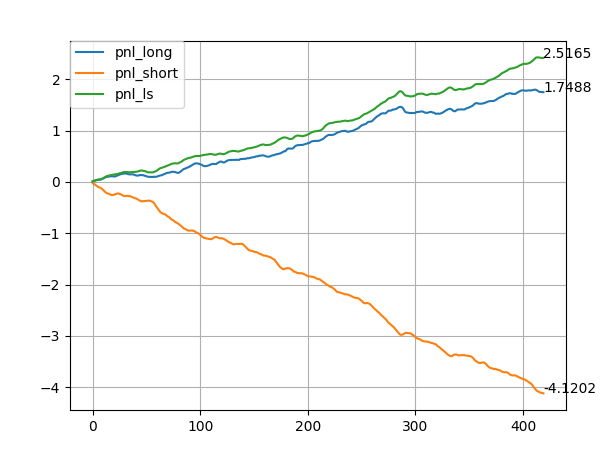
\includegraphics[width=0.8\textwidth]{plt2.PNG}
\end{center}
\caption{model31 pnl figure}
\label{FIG.1}
\end{figure}

原有模型:
{\kaishu \small IC\_old: 0.065, pnl\_old:2.1}

\subsection{2.新的时间序列观点的引入}
新的时间序列观点是基于日频信号的生成逻辑。上面的操作是将bar数据直接带入模型,现在想在模型上添加日频信号观点。所以,先将数据切分成10份,代表十天,然后将每天的数据分别带入模型计算结果,最后将数据结果cat在一起合成总的结果。再和上面的模型结果相加。具体操作有两种:

1.将每日数据取平均,然后将seqlength=10的日数据带入同种模型,最后和原来的分钟结果相加。

2.将每日数据分别带入模型,然后cat在一起,最后和原来的分钟结果相加。

经过改造的模型也采用修正的模型,保证时间长度相等。其结果如下:

模型1:普通CNN2d(ordinary*2+pointwise+linear*2+dropout+relu)

{\kaishu \small IC: 0.062, pnl:2.2}

原有模型:
{\kaishu \small IC\_old: 0.056, pnl\_old:1.9}

由此可见,从最基础的模型开始,加入新观点的模型解释能力有了实质的提高。虽然训练时间增长,但是效果显著,同时没有观察到模型复杂产生的快速过拟合情况发生。

~\\
模型2:普通CNN2d(deepwise*2+pointwise+linear*2+dropout+relu)

{\kaishu \small IC: 0.062, pnl:2.25}

原有模型:
{\kaishu \small IC\_old: 0.056, pnl\_old:1.9}

~\\
模型3:普通CNN2d(ordinary*2+linear*2+pointwise+linear*2+dropout+relu)

{\kaishu \small IC: 0.053, pnl:1.8}

原有模型:
{\kaishu \small IC\_old: 0.046, pnl\_old:1.9}

~\\
模型4:普通CNN2d(deepwise*2+linear*2+pointwise+linear*2+dropout+relu)

{\kaishu \small IC: 0.066, pnl:2.3}

原有模型:
{\kaishu \small IC\_old: 0.056, pnl\_old:1.9}

~\\
模型5:普通CNN2d(deepwise*2+maxpool+linear*2+pointwise+linear*2+dropout+relu)

{\kaishu \small IC: 0.052, pnl:2.3}

原有模型:
{\kaishu \small IC\_old: 0.041, pnl\_old:1.7}

~\\
模型6:普通CNN2d(deepwise*2+ordinary+linear*2+pointwise+linear*2+dropout+relu)

{\kaishu \small IC: 0.058, pnl:2.2}

原有模型:
{\kaishu \small IC\_old: 0.065, pnl\_old:2.1}

~\\
模型7:普通CNN2d(deepwise*2+ordinary*3+linear*2+pointwise+linear*2+dropout+relu)

{\kaishu \small IC: 0.069, pnl:2.4}

原有模型:
{\kaishu \small IC\_old: 0.065, pnl\_old:2.1}

~\\
模型8:普通CNN1d(ordinary*2+avg+linear*2+dropout+relu)

{\kaishu \small IC: 0.047, pnl:2.0}

原有模型:
{\kaishu \small IC\_old: 0.044, pnl\_old:1.9}

对于cnn1d而言,时间处理方式不太相同,但是大同小异。面对复杂的模型,后面有专门交代
~\\
模型9:普通CNN1d(ordinary*2+avg+ordinary*2+linear*2+dropout+relu)

{\kaishu \small IC: 0.056, pnl:2.1}

原有模型:
{\kaishu \small IC\_old: 0.045, pnl\_old:2.0}

~\\
模型10:普通CNN1d(ordinary*2+avg+ordinary*2+linear*2+pointwise+dropout+relu)

{\kaishu \small IC: 0.055, pnl:2.5}

原有模型:
{\kaishu \small IC\_old: 0.045, pnl\_old:1.8}

模型10表现较好。原有模型表现较差。但是并未观察到数据过拟合的特征。

~\\
模型11:普通CNN1d((ordinary+avg+relu)*3+(ordinary+relu)*2+ordinary+linear*2+dropout+relu)

{\kaishu \small IC: 0.057, pnl:2.0}

原有模型:
{\kaishu \small IC\_old: 0.053, pnl\_old:2.0}

~\\
模型12:普通CNN1d((ordinary+avg+relu)*3+(ordinary+relu)*3+ordinary+linear*2+dropout+relu)

{\kaishu \small IC: 0.051, pnl:2.0}

原有模型:
{\kaishu \small IC\_old: 0.049, pnl\_old:2.0}

~\\
模型13:普通CNN1d((ordinary+avg+relu)*4+(ordinary+relu)*3+ordinary+linear*2+dropout+relu)

{\kaishu \small IC: 0.051, pnl:2.3}

原有模型:
{\kaishu \small IC\_old: 0.049, pnl\_old:2.0}

~\\
模型14:普通CNN1d((ordinary+avg+relu)*5+(ordinary+relu)*3+ordinary+linear*2+dropout+relu)

{\kaishu \small IC: 0.051, pnl:2.15}

原有模型:
{\kaishu \small IC\_old: 0.056, pnl\_old:2.1}

~\\
模型15:普通CNN1d((ordinary+avg+relu)*6+(ordinary+relu)*3+ordinary+linear*2+dropout+relu)

{\kaishu \small IC: 0.073, pnl:2.58}

原有模型:
{\kaishu \small IC\_old: 0.056, pnl\_old:2.1}

~\\
模型16:bottleneck((cnn1d(1)+cnn1d(3)+cnn1d(1))+pointwise+linear+dropout+relu)

{\kaishu \small IC: 0.047, pnl:1.8}

原有模型:
{\kaishu \small IC\_old: 0.058, pnl\_old:1.8}

~\\
模型17:bottleneck((cnn1d(1)+cnn1d(3)+cnn1d(1))+pointwise+linear+dropout+relu)


{\kaishu \small IC: 0.046, pnl:1.6}

原有模型:
{\kaishu \small IC\_old: 0.061, pnl\_old:1.9}

~\\
模型18:base((cnn1d+batchnorm+relu+avgpool)*2+pointwise+linear+dropout+relu)

{\kaishu \small IC: 0.043, pnl:1.7}

原有模型:
{\kaishu \small IC\_old: 0.031, pnl\_old:1.4}

~\\
模型19: bottleneck((cnn1d+batchnorm+relu+avgpool)*2+bottleneck1+pointwise

+linear+dropout+relu)

{\kaishu \small IC: 0.042, pnl:1.6}

原有模型:
{\kaishu \small IC\_old: 0.045, pnl\_old:1.8}

~\\
模型20: bottleneck((cnn1d+batchnorm+relu+avgpool)*2+bottleneck2+pointwise

+linear+dropout+relu)

{\kaishu \small IC: 0.046, pnl:1.6}

原有模型:
{\kaishu \small IC\_old: 0.046, pnl\_old:1.6}

可以看出,在模型18和19上序列缩短效果较好。

~\\
模型21: bottleneck((cnn1d+batchnorm+relu+avgpool)*2+bottleneck1+bottleneck2+pointwise

+linear+dropout+relu)

{\kaishu \small IC: 0.045, pnl:1.4}

原有模型:
{\kaishu \small IC\_old: 0.048, pnl\_old:1.9}

从模型21开始恢复正常,修正模型的效果稍微强一点。

~\\
模型22: deepnn((cnn1d+batchnorm+relu+avgpool)*2+bottleneck1

+bottleneck2+bottleneck1+bottleneck2+pointwise+linear+dropout+relu)

{\kaishu \small IC: 0.069, pnl:2.0}

原有模型:
{\kaishu \small IC\_old: 0.065, pnl\_old:2.1}

~\\
模型23: multigrid(base+multigrid+poitwise)

{\kaishu \small IC: 0.073, pnl:2.3}

原有模型:
{\kaishu \small IC\_old: 0.069, pnl\_old:2.2}

~\\
模型24: multigrid+bottleneck(base+bottleneck+multigrid\_assp+linear)

{\kaishu \small IC: 0.071, pnl:2.3}

原有模型:
{\kaishu \small IC\_old: 0.065, pnl\_old:2.1}

~\\
模型25:multigrid+bottleneck(base+bottleneck+multigrid\_batchnorm+linear)

{\kaishu \small IC: 0.072, pnl:2.3}

原有模型:
{\kaishu \small IC\_old: 0.065, pnl\_old:2.1}

~\\26:multigrid+bottleneck(base+bottleneck+multigrid\_batchnorm+linear)

计算出的结果还是一样。

{\kaishu \small IC: 0.072, pnl:2.3}

原有模型:
{\kaishu \small IC\_old: 0.071, pnl\_old:2.4}

~\\
模型27:multigrid+bottleneck(base+bottleneck+multigrid\_batchnorm+linear)

{\kaishu \small IC: 0.068, pnl:2.1}

原有模型:
{\kaishu \small IC\_old: 0.065, pnl\_old:2.1}

~\\
模型28:multigrid+bottleneck(base+bottleneck+multigrid\_batchnorm+downsample)

{\kaishu \small IC: 0.064, pnl:2.1}

原有模型:
{\kaishu \small IC\_old: 0.064, pnl\_old:2.1}

~\\
模型29:multigrid(multigrid\_batchnorm+downsample)

{\kaishu \small IC: 0.070, pnl:2.45}

原有模型:
{\kaishu \small IC\_old: 0.071, pnl\_old:2.2}

~\\
模型30:multigrid(multigrid\_batchnorm+downsample+upsample)

{\kaishu \small IC: 0.070, pnl:2.3}

原有模型:
{\kaishu \small IC\_old: 0.065, pnl\_old:2.1}

~\\
模型31:multigrid(multigrid\_batchnorm+downsample+upsample)

{\kaishu \small IC: 0.078, pnl:2.45}

\begin{figure}[H]
\begin{center}
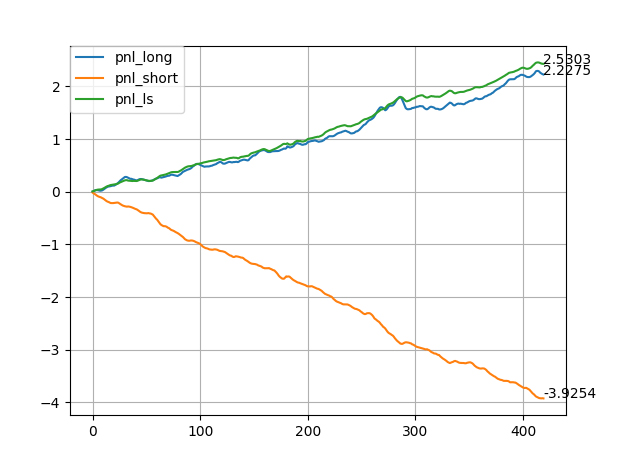
\includegraphics[width=0.8\textwidth]{plt3.PNG}
\end{center}
\caption{model31 pnl figure}
\label{FIG.2}
\end{figure}

原有模型:
{\kaishu \small IC\_old: 0.065, pnl\_old:2.1}

\subsection{3.三种思路和对比和总结}

\begin{longtable}[tbp]{|l|l|l|l|}
\hline
model\_name/pnl                                                                                                                                                      & 原始模型 & 修正模型 & 加时间序列观点 \\ \hline
\begin{tabular}[c]{@{}l@{}}普通CNN2d(ordinary*2+pointwise+\\ linear*2+dropout+relu)\end{tabular}                                                                       & 1.9  & 2.0  & 2.2     \\ \hline
\begin{tabular}[c]{@{}l@{}}普通CNN2d(deepwise*2+pointwise+\\ linear*2+dropout+relu)\end{tabular}                                                                       & 1.9  & 2.1  & 2.25    \\ \hline
\begin{tabular}[c]{@{}l@{}}普通CNN2d(ordinary*2+linear*2+\\ pointwise+linear*2+dropout+relu)\end{tabular}                                                              & 1.9  & 1.9  & 2.8     \\ \hline
\begin{tabular}[c]{@{}l@{}}普通CNN2d(deepwise*2+linear*2+\\ pointwise+linear*2+dropout+relu)\end{tabular}                                                              & 2.0  & 1.9  & 2.3     \\ \hline
\begin{tabular}[c]{@{}l@{}}普通CNN2d(deepwise*2+maxpool+\\ linear*2+pointwise+linear*2+dropout+relu)\end{tabular}                                                      & 1.7  & 1.8  & 2.3     \\ \hline
\begin{tabular}[c]{@{}l@{}}普通CNN2d(deepwise*2+ordinary+\\ linear*2+pointwise+linear*2+dropout+relu)\end{tabular}                                                     & 2.2  & 2.1  & 2.4     \\ \hline
\begin{tabular}[c]{@{}l@{}}普通CNN2d(deepwise*2+ordinary*3+\\ linear*2+pointwise+linear*2+dropout+relu)\end{tabular}                                                   & 2.1  & 2.4  & 2.5     \\ \hline
\begin{tabular}[c]{@{}l@{}}普通CNN1d(ordinary*2+avg+ordinary*2+\\ linear*2+dropout+relu)\end{tabular}                                                                  & 1.9  & 2.0  & 1.9     \\ \hline
\begin{tabular}[c]{@{}l@{}}普通CNN1d(ordinary*2+avg+ordinary*2+\\ linear*2+pointwise+dropout+relu)\end{tabular}                                                        & 1.8  & 1.9  & 2.1     \\ \hline
\begin{tabular}[c]{@{}l@{}}普通CNN1d((ordinary+avg+relu)*3+\\ (ordinary+relu)*2+ordinary+linear*2+\\ dropout+relu)\end{tabular}                                        & 1.8  & 2.0  & 2.5     \\ \hline
\begin{tabular}[c]{@{}l@{}}普通CNN1d((ordinary+avg+relu)*3+\\ (ordinary+relu)*3+ordinary+linear*2+\\ dropout+relu)\end{tabular}                                        & 2.0  & 2.0  & 2.0     \\ \hline
\begin{tabular}[c]{@{}l@{}}普通CNN1d((ordinary+avg+relu)*4+\\ (ordinary+relu)*3+ordinary+linear*2+\\ dropout+relu)\end{tabular}                                        & 2.0  & 2.1  & 2.3     \\ \hline
\begin{tabular}[c]{@{}l@{}}普通CNN1d((ordinary+avg+relu)*5+\\ (ordinary+relu)*3+ordinary+linear*2+\\ dropout+relu)\end{tabular}                                        & 2.1  & 2.25 & 2.15    \\ \hline
\begin{tabular}[c]{@{}l@{}}普通CNN1d((ordinary+avg+relu)*6+\\ (ordinary+relu)*3+ordinary+linear*2+\\ dropout+relu)\end{tabular}                                        & 2.1  & 2.42 & 2.58    \\ \hline
\begin{tabular}[c]{@{}l@{}}bottleneck((cnn1d(1)+cnn1d(3)+cnn1d(1))+\\ pointwise+linear+dropout+relu)\end{tabular}                                                    & 1.7  & 1.8  & 2.1     \\ \hline
\begin{tabular}[c]{@{}l@{}}bottleneck((cnn1d(1)+cnn1d(3)+cnn1d(1))+\\ pointwise+linear+dropout+relu)\end{tabular}                                                    & 1.7  & 1.9  & 1.9     \\ \hline
\begin{tabular}[c]{@{}l@{}}base((cnn1d+batchnorm+relu+avgpool)*2+\\ pointwise+linear+dropout+relu)\end{tabular}                                                      & 1.4  & 1.4  & 1.6     \\ \hline
\begin{tabular}[c]{@{}l@{}}bottleneck((cnn1d+batchnorm+relu+avgpool)*2+\\ bottleneck1+pointwise+linear+dropout+relu)\end{tabular}                                    & 1.5  & 1.8  & 1.7     \\ \hline
\begin{tabular}[c]{@{}l@{}}bottleneck((cnn1d+batchnorm+relu+avgpool)*2+\\ bottleneck2+pointwise+linear+dropout+relu)\end{tabular}                                    & 1.37 & 1.6  & 1.4     \\ \hline
\begin{tabular}[c]{@{}l@{}}bottleneck((cnn1d+batchnorm+relu+avgpool)*2+\\ bottleneck1+bottleneck2+pointwise+linear+\\ dropout+relu)\end{tabular}                     & 1.4  & 1.9  & 1.6     \\ \hline
\begin{tabular}[c]{@{}l@{}}deepnn((cnn1d+batchnorm+relu+avgpool)*2+\\ bottleneck1+bottleneck2+bottleneck1+\\ bottleneck2+pointwise+linear+dropout+relu)\end{tabular} & 2.0  & 2.1  & 2.0     \\ \hline
multigrid(base+multigrid+poitwise)                                                                                                                                   & 2.3  & 2.2  & 2.3     \\ \hline
\begin{tabular}[c]{@{}l@{}}multigrid+bottleneck(base+bottleneck+\\ multigrid\_assp+linear)\end{tabular}                                                              & 2.4  & 2.1  & 2.3     \\ \hline
\begin{tabular}[c]{@{}l@{}}multigrid+bottleneck(base+bottleneck+\\ multigrid\_batchnorm+linear)\end{tabular}                                                         & 2.3  & 2.1  & 2.3     \\ \hline
\begin{tabular}[c]{@{}l@{}}multigrid+bottleneck(base+bottleneck+\\ multigrid\_batchnorm+linear)\end{tabular}                                                         & 2.4  & 2.5  & 2.3     \\ \hline
\begin{tabular}[c]{@{}l@{}}multigrid+bottleneck(base+bottleneck+\\ multigrid\_batchnorm+linear)\end{tabular}                                                         & 2.1  & 2.1  & 2.3     \\ \hline
\begin{tabular}[c]{@{}l@{}}multigrid+bottleneck(base+bottleneck+\\ multigrid\_batchnorm+downsample)\end{tabular}                                                     & 2.1  & 2.1  & 2.1     \\ \hline
multigrid(multigrid\_batchnorm+downsample)                                                                                                                           & 2.2  & 2.45 & 2.53    \\ \hline
\begin{tabular}[c]{@{}l@{}}multigrid(multigrid\_batchnorm+\\ downsample+upsample)\end{tabular}                                                                       & 2.3  & 2.1  & 2.53    \\ \hline
\begin{tabular}[c]{@{}l@{}}multigrid(multigrid\_batchnorm+\\ downsample+upsample)\end{tabular}                                                                       & 2.45 & 2.58 & 2.46    \\ \hline
\end{longtable}


\subsection{4.改进思路}
\begin{itemize}
  \item [0)]
  对原来的模型框架进行了整个修改和重置。我觉得在这些模型上能取得的效果已经尽可能发掘了。单纯从CNN提取信息的角度感觉很难发掘出新的东西。下面一部就是开发新的模型,采取新的思路,从CNN目标检测的角度入手,选取取景框,采用回归算法对取景框进行修正,检测是否有某种信号的产生。常用成熟的模型有multibox,yolo系列,fastRCNN等。下一步从这个角度入手深入研究CNN系列模型。
\end{itemize}


\section{第三、RNN的研究:convolutedRNNcell}
\subsection{综述}
RNN的研究基于老的已经设计的RNNcell来进行,首先,原来的RNN每个门不再采用多个线性网络的结构。而是采用一个线性网络。这个线性网络的输入通道数是hidden\_state+cell\_state+x。输出的通道数是门数量*output\_channel。将多个门并在一起,同时进行线性前馈网络。大大减少了所需要的时间。在操作的最后,采用torch.split系列操作将一个大的线性层分割成几个小的线性层。找到输入和输出。这样做的另一个好处是方便进行卷积研究。可以在大的多通道上进行卷积和pooling,不再拘泥于每个门对应多个线性层,不同的特征之间也可以算出仙湖关系,注意力,卷积等。结果如下:
\begin{figure}[H]
\begin{center}
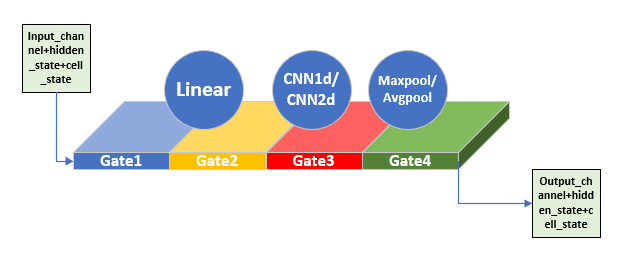
\includegraphics[width=0.8\textwidth]{str1.PNG}
\end{center}
\caption{new rnncell structure}
\label{FIG.3}
\end{figure}
对所有RNNcell进行了改写。同时设计了multilayer多层联动装置。保证RNNcell可以自由地串并联,彻底改革了代码结构。不再需要cell之间复杂的数据交换,只需要将cell的种类和层数,串并联图的结构输入即可。

因此,基于新的结构和新的cell做了如下设计。
\subsection{newcell结构}

\subsubsection{convGRU}
convGRU的意义在于,根据GRU的公式,需要做两次线性层,第一次分割成r,z两个门,第二次用r*hidden\_state形成n也就是第二次线性层。那么可以将这两次线性层替换成卷积层convolution.结构如下:
\begin{figure}[H]
\begin{center}
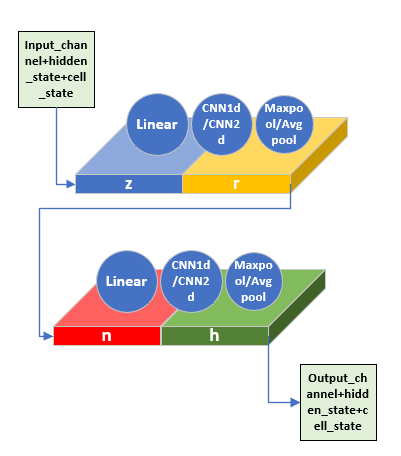
\includegraphics[width=0.7\textwidth]{str5.PNG}
\end{center}
\caption{conv GRU structure}
\label{FIG.4}
\end{figure}

注意,替换的本意有两个,一是对截面进行卷积,学习截面的结构,提取截面的特征,然后带入GRU看特征的变化。这样batch\_size就必须是提前加入的1.kernel\_size可以是任意的数。第二种是对单个元素做pointwise的卷积,这之后batch\_size就还是原来的batch\_size,但是kernel只能是1。因此有这两种替换方式,要分别设计模型。

模型1:convGRU(conv+linear)\_2layer(layer1(batch:1,kernel:3), layer2(batch:1,kernel:3)) 替换第一个线性层为卷积

{\kaishu \small IC: 0.047, pnl:2.1}

~\\
模型2:convGRU(conv+linear)\_2layer(layer1(batch:n,kernel:1), layer2(batch:n,kernel:1)) 替换第一个线性层为卷积

{\kaishu \small IC: 0.037, pnl:1.8}
可以看到两层都是1 batch的表现好于两层都是n batch的表现,两层都是n batch的表现使用了poitwise增加了过拟合

~\\
模型3:convGRU(conv+linear)\_2layer(layer1(batch:n,kernel:1), layer2(batch:1,kernel:3)) 替换第一个线性层为卷积

{\kaishu \small IC: 0.048, pnl:2.2}

两层交叉进行,表现比前两次都好,类似于先卷积给出序列观点,再用pointwise给出界面观点

将两层都换成convolution,效果又强于上面改动的结果。

~\\
模型4:convGRU(conv+conv)\_2layer(layer1(batch:1,kernel:3), layer2(batch:1,kernel:3)) 替换两个线性层为卷积

{\kaishu \small IC: 0.057, pnl:2.2}

~\\
模型5:convGRU(conv+conv)\_2layer(layer1(batch:n,kernel:1), layer2(batch:n,kernel:1)) 替换两个线性层为卷积

{\kaishu \small IC: 0.048, pnl:1.9}

~\\
模型6:convGRU(conv+conv)\_2layer(layer1(batch:n,kernel:1), layer2(batch:1,kernel:3)) 替换两个线性层为卷积

{\kaishu \small IC: 0.063, pnl:2.4}

将第二层换成convolution,效果又强于上面改动的结果。

~\\
模型7:convGRU(linear+conv)\_2layer(layer1(batch:1,kernel:3), layer2(batch:1,kernel:3)) 替换第二个线性层为卷积

{\kaishu \small IC: 0.054, pnl:2.1}

~\\
模型8:convGRU(linear+conv)\_2layer(layer1(batch:n,kernel:1), layer2(batch:n,kernel:1)) 替换第二个线性层为卷积

{\kaishu \small IC: 0.055, pnl:2.3}

~\\
模型9:convGRU(linear+conv)\_2layer(layer1(batch:n,kernel:1), layer2(batch:1,kernel:3)) 替换第二个线性层为卷积

{\kaishu \small IC: 0.060, pnl:2.0}

~\\
模型10:convGRU(conv+conv)\_4layer(layer1(batch:n,kernel:1), layer2(batch:n,kernel:1), layer3(batch:1, kernel:3),layer4(batch:1, kernel:3)) 替换两层为卷积

{\kaishu \small IC: 0.069, pnl:2.5}
模型10是在convGRUcell里实验出的表现最好的模型。
\begin{figure}[H]
\begin{center}
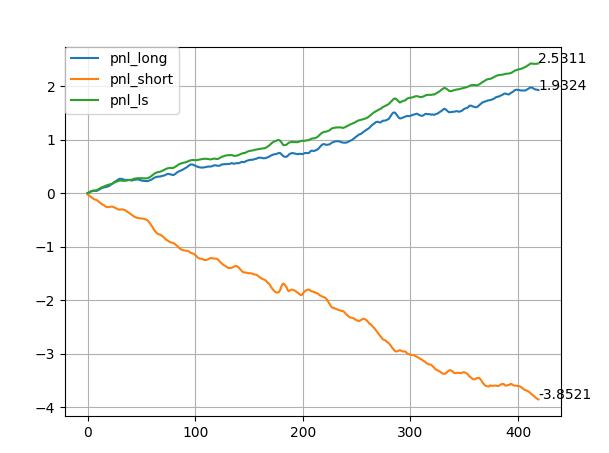
\includegraphics[width=0.8\textwidth]{plt4.PNG}
\end{center}
\caption{convGRU best pnl figure}
\label{FIG.5}
\end{figure}


\subsubsection{convLSTM}
convLSTM的意义在于,根据LSTM的公式,需要做一次线性层,那么可以将线性层替换成卷积层convolution.结构和最基础的结构一样。如下图:
\begin{figure}[H]
\begin{center}
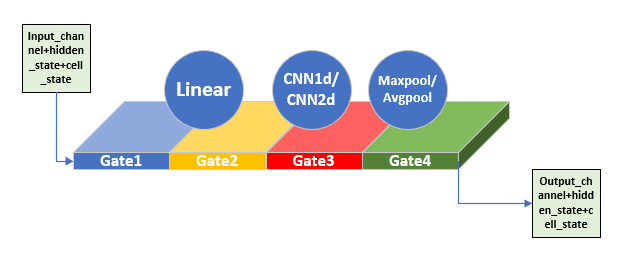
\includegraphics[width=0.8\textwidth]{str1.PNG}
\end{center}
\caption{convLSTM structure figure}
\label{FIG.6}
\end{figure}

模型1:convLSTM(conv)\_2layer(layer1(batch:1,kernel:3), layer2(batch:1,kernel:3))

{\kaishu \small IC: 0.055, pnl:2.5}

~\\
模型2:convGRU(conv)\_2layer(layer1(batch:n,kernel:1), layer2(batch:n,kernel:1))

{\kaishu \small IC: 0.053, pnl:2.3}

~\\
模型3:convGRU(conv)\_2layer(layer1(batch:n,kernel:1), layer2(batch:1,kernel:3))

{\kaishu \small IC: 0.058, pnl:2.4}


\subsubsection{convRNN}
convRNN的意义在于,根据RNN的公式,需要做一次线性层,那么可以将线性层替换成卷积层convolution.结构和最基础的结构一样。

模型1:convRNN(conv)\_2layer(layer1(batch:1,kernel:3), layer2(batch:1,kernel:3))

{\kaishu \small IC: 0.052, pnl:2.1}

~\\
模型2:convRNN(conv)\_2layer(layer1(batch:n,kernel:1), layer2(batch:n,kernel:1))

{\kaishu \small IC: 0.049, pnl:2.0}

~\\
模型3:convRNN(conv)\_2layer(layer1(batch:n,kernel:1), layer2(batch:1,kernel:3))

{\kaishu \small IC: 0.047, pnl:2.0}

只尝试了最简单的情况,后面继续尝试增加层数


\subsubsection{convLSTMC}
convLSTMC的意义在于,根据LSTMC的公式,需要做一次线性层,那么可以将线性层替换成卷积层convolution.结构和最基础的结构一样。

模型1:convLSTMC(conv)\_2layer(layer1(batch:1,kernel:3), layer2(batch:1,kernel:3))

{\kaishu \small IC: 0.051, pnl:2.1}

~\\
模型2:convLSTMC(conv)\_2layer(layer1(batch:n,kernel:1), layer2(batch:n,kernel:1))

{\kaishu \small IC: 0.045, pnl:2.1}

~\\
模型3:convLSTMC(conv)\_2layer(layer1(batch:n,kernel:1), layer2(batch:1,kernel:3))

{\kaishu \small IC: 0.044, pnl:2.1}

只尝试了最简单的情况,后面继续尝试增加层数


\subsubsection{conv\_passcell\_1}
conv\_passcell\_1的意义在于,根据conv\_passcell\_1的公式,需要做一次线性层,那么可以将线性层替换成卷积层convolution.结构和最基础的结构一样。

模型1:conv\_passcell\_1(conv)\_2layer(layer1(batch:1,kernel:3), layer2(batch:1,kernel:3))

{\kaishu \small IC: 0.052, pnl:2.1}

~\\
模型2:conv\_passcell\_1(conv)\_2layer(layer1(batch:n,kernel:1), layer2(batch:n,kernel:1))

{\kaishu \small IC: 0.049, pnl:2.0}

~\\
模型3:conv\_passcell\_1(conv)\_2layer(layer1(batch:n,kernel:1), layer2(batch:1,kernel:3))

{\kaishu \small IC: 0.047, pnl:2.0}

只尝试了最简单的情况,后面继续尝试增加层数


\subsubsection{conv\_passcell\_2}
conv\_passcell\_2的意义在于,根据conv\_passcell\_2的公式,需要做两次线性层,第一次分割成一个门,第二次用x,hidden\_state,cell\_state形成第二次线性层。那么可以将这两次线性层替换成卷积层convolution.结构如下:
\begin{figure}[H]
\begin{center}
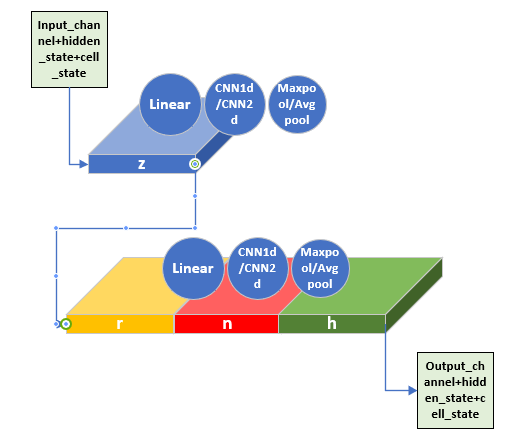
\includegraphics[width=0.8\textwidth]{str6.PNG}
\end{center}
\caption{conv\_passcell\_2 structure}
\label{FIG.7}
\end{figure}

注意,替换的还是有两个,第一是对截面进行卷积,第二种是对单个元素做pointwise的卷积。因此有这两种替换方式,要分别设计模型。

模型1:conv\_passcell\_2(conv+linear)\_2layer(layer1(batch:1,kernel:3), layer2(batch:1,kernel:3)) 替换第一个线性层为卷积

{\kaishu \small IC: 0.061, pnl:2.2}

~\\
模型2:conv\_passcell\_2(conv+linear)\_2layer(layer1(batch:n,kernel:1), layer2(batch:n,kernel:1)) 替换第一个线性层为卷积

{\kaishu \small IC: 0.064, pnl:2.3}
可以看到两层都是1 batch的表现好于两层都是n batch的表现,两层都是n batch的表现使用了poitwise增加了过拟合

~\\
模型3:conv\_passcell\_2(conv+linear)\_2layer(layer1(batch:n,kernel:1), layer2(batch:1,kernel:3)) 替换第一个线性层为卷积

{\kaishu \small IC: 0.068, pnl:2.4}

两层交叉进行,表现比前两次都好,类似于先卷积给出序列观点,再用pointwise给出界面观点

将两层都换成convolution,效果又强于上面改动的结果。

~\\
模型4:conv\_passcell\_2(conv+conv)\_2layer(layer1(batch:1,kernel:3), layer2(batch:1,kernel:3)) 替换两个线性层为卷积

{\kaishu \small IC: 0.067, pnl:2.25}

~\\
模型5:conv\_passcell\_2(conv+conv)\_2layer(layer1(batch:n,kernel:1), layer2(batch:n,kernel:1)) 替换两个线性层为卷积

{\kaishu \small IC: 0.068, pnl:2.4}

~\\
模型6:conv\_passcell\_2(conv+conv)\_2layer(layer1(batch:n,kernel:1), layer2(batch:1,kernel:3)) 替换两个线性层为卷积

{\kaishu \small IC: 0.063, pnl:2.3}

将第二层换成convolution,效果又强于上面改动的结果。

~\\
模型7:conv\_passcell\_2(linear+conv)\_2layer(layer1(batch:1,kernel:3), layer2(batch:1,kernel:3)) 替换第二个线性层为卷积

{\kaishu \small IC: 0.057, pnl:2.0}

~\\
模型8:conv\_passcell\_2(linear+conv)\_2layer(layer1(batch:n,kernel:1), layer2(batch:n,kernel:1)) 替换第二个线性层为卷积

{\kaishu \small IC: 0.056, pnl:2.0}

~\\
模型9:conv\_passcell\_2(linear+conv)\_2layer(layer1(batch:n,kernel:1), layer2(batch:1,kernel:3)) 替换第二个线性层为卷积

{\kaishu \small IC: 0.059, pnl:2.05}


\section{第四、baseline model,序列分类网络}
\subsection{综述}
意识到目前的序列截面观点任务其实是一个序列分类任务以后,很容易想到利用BERT model进行序列分类。在NLP里,其实关于序列一共有五种任务,分别是文本分类(常用的模型有:Fast text, ReNN,MLP,RNN,CNN,Attention,Transformer)。 句子间匹配\par (常用的模型是representation based和interaction based),序列标注(常见的模型是embedding module,context encoder),文本生成,以及语言模型。虽然一共只有五种任务,但是具体到不同的场景,方案是很复杂的,开始深入到一个具体的场景,根据不同的case创造自己的解决方案。

因此,在这个任务中,我目前看到了第一层,序列分类任务。序列分类任务常用的模型有(DecAtt,PWIM,  MatchPyramid, ESIM,DIIN,BERT,HCAN,RE2)由于我只对BERT有所了解,所以采用BERT模型进行操作。BERT模型其实是多层transformer encoder堆叠而成,每一层的encoder的结果输入到下一层中,经过多层encoder输出理解过的序列。\par每个encoder其实是6层transformerencoderlayer构成,因子在每一个encoder里面,先进行数据运算,重复多次后,进入下一个encoder。为了防止模型变现变差,加入了resnet进行调节。

transformer模型的意义在于计算每两个时间点之间的内积作为attention,经过前馈神经网络传递到最后。为了保证序列的先后顺序被记住,采用了positional encoding的办法。为了获得对整个序列的理解,采用了SEP和CLS向量作为整个序列的理解。 CLS向量全称是classification,是用一个头部张量来理解整个句子,在实际计算中,cls张量会和整个句子计算attention并且他的结果会保留输出到下一层。经过多层和多次梯度下降,cls越来越接近整个句子的理解。SEP向量放在句子的尾部,一般用作分割句子和句子衔接的作用,那么,sep向量和cls向量有共同或者相近的含义时,可以认为句子是良好衔接的。因此用sep也作为分类的一个标准,增加了模型的鲁棒性。

下面这张图解释了transformer attention的操作机制:
\begin{figure}[H]
\begin{center}
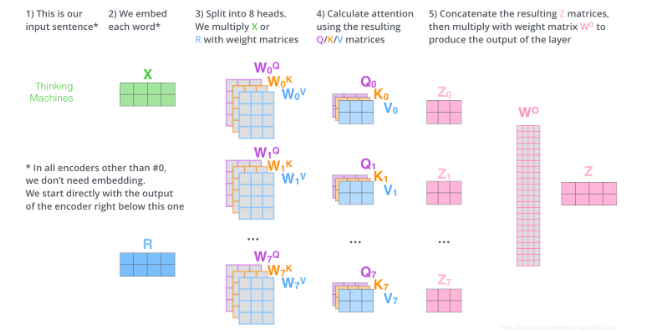
\includegraphics[width=1.0\textwidth]{str3.PNG}
\end{center}
\caption{transformer encoder layer structure}
\label{FIG.8}
\end{figure}
这张 图是解释的最全的multi-head self attention机制。

这张图解释了bert模型的机制和cls向量的作用。
\begin{figure}[H]
\begin{center}
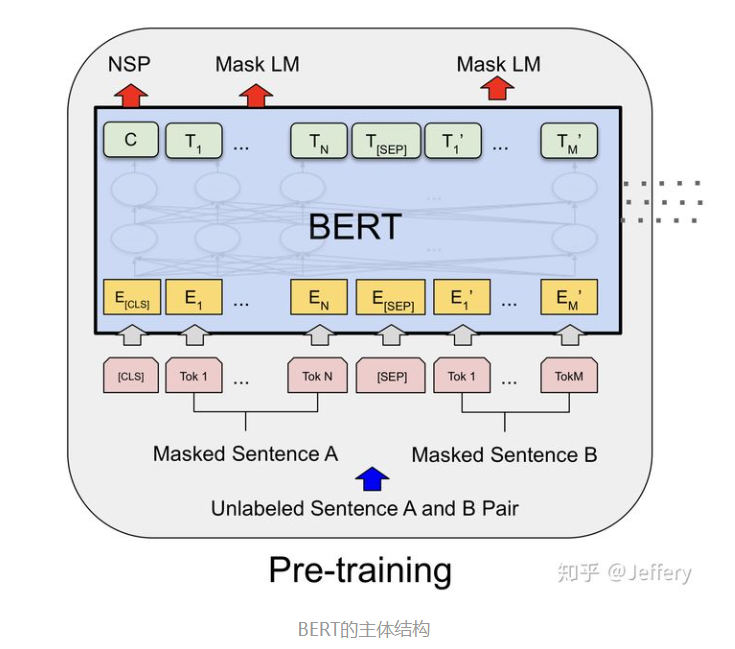
\includegraphics[width=0.8\textwidth]{str4.PNG}
\end{center}
\caption{BERT structure}
\label{FIG.9}
\end{figure}
在图中,每个token就是一个时间序列点,最头部时cls向量,代表整个句子含义,最后面加上sep向量,代表句子衔接含义。BERT就是多层transformer encoder的串联。

\subsection{实验}
由于算力减半,目前模型待跑,设计了以下几种模型

模型1: tansformer(1 layer* 1 encoder) + resnet head = 1

{\kaishu \small IC: 0.026, pnl:1.3}

\begin{figure}[H]
\begin{center}
\includegraphics[width=0.8\textwidth]{plt\_box.PNG}
\end{center}
\caption{transformer模型 pnl图}
\label{FIG.10}
\end{figure}
发现,这个方法的多头和空头和以往的RNN和CNN模型的多头和空头正好反过来。说明开发到了新的特征,虽然表现不好,但是这也只是简单的模型,后面可以对这个方向深入挖掘。

模型2: transformer( 3 layer* 1 encoder) +resnet head = 1模型待跑
模型3: transformer( 3 layer* 3 encoder) +resnet head = 1模型待跑
模型4: transformer( 6 layer* 1 encoder) +resnet head = 1模型待跑
模型5: transformer( 6 layer* 6 encoder) +resnet head = 1模型待跑
由于目前的输入维度是3,因此num\_head的数目只能是1或3.对于三天head相当于把三个维度全部分割,个人感觉效果应该不好,后面可以做相应的尝试。

\subsection{讨论}
虽然结果不好,但是惊奇的发现pnl图反了过来。说明这是一个不同于以往的特征提取方式。因此这个角度可以深入挖掘。对于序列分类任务,\par 还有(DecAtt,PWIM,  MatchPyramid, ESIM,DIIN,BERT,HCAN,RE2)的模型可以尝试,本质上都是基于transformer。此外,目前采用的是cls和sep向量直接作为句子的观点。本身还可以给这两个向量添加操作,或者使用多个观点向量,后面会继续探索。


\section{第五、基于multibox detector的目标检测网络}
\subsection{综述}
目标检测网络主要是应用于数据上找到特定信号,instancewise的网络结构。目前有三大网络结构,fastRCNN,multibox detector和yolo。我这段时间着重研究了fast RCNN和multibox detector,FastRCNN的结构如下:

首先从三层convolution网络中提取信息,将futuremap分成两部分,一部分用于区域CNN网络,另一部分经过pooling到达分类器,最后两部分的结果相加。相当于选取区域和区域内容两部分观点。区域CNN网络是采用adaptiveCNN和adaptivepooling的方法,先在数据上随即选取区域,然后用adaptive的CNN和pooling层在区域上进行特征提取。提取的结果数据大小窗口也是随机的,然后再用同一大小的CNN窗口进行特征提取。将不同大小的窗口都换算成数量不等的多个窗口。接着,再与另一部分分类提取相加。得到最后的结果。结构图如下图:
\begin{figure}[H]
\begin{center}
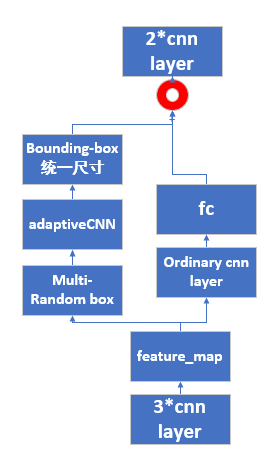
\includegraphics[width=0.5\textwidth]{str2.PNG}
\end{center}
\caption{multibox detector structure}
\label{FIG.11}
\end{figure}

计算结果:
\begin{figure}[H]
\begin{center}
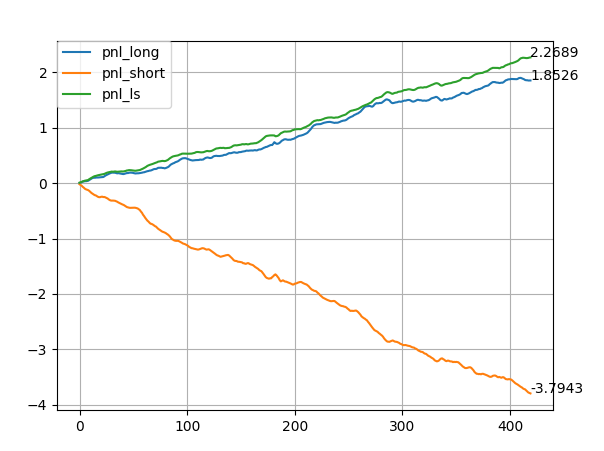
\includegraphics[width=0.8\textwidth]{plt1.PNG}
\end{center}
\caption{fasterRCNN pnl figure}
\label{FIG.12}
\end{figure}
FastRCNN存在对于小的目标不敏感,检测不到,以及对于整体的趋势检测很慢的特点。因此更多的采用multibox detector模型。multibox模型不再采用随机选取的检测框。因为随即检测框不仅要求识别和分类,还要具体的框出来。而multibox只需要进行检测就可以。所以,直接在不同目标尺度上进行预测就可以。

首先,先经过三层CNN网络生成三层feature\_map,然后和fasterRCNN的结果一样,直接作为结果的一部分。然后将结果用缩小一半的序列重新表出,再进行特征提取。每次特征提取都要加上resnet和全连接网络。然后,再次重复这个过程,让尺度继续缩小,直到缩小到尺度为3的网络应用最后一次卷积。将所有的结果取attention作用到截面上。效果如图所示:
\begin{figure}[H]
\begin{center}
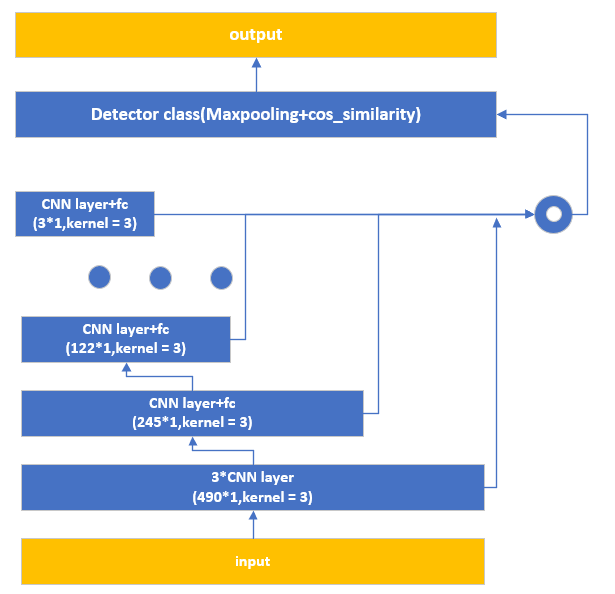
\includegraphics[width=0.8\textwidth]{str7.PNG}
\end{center}
\caption{multibox detector figure}
\label{FIG.13}
\end{figure}

\subsection{讨论}
目前还没有大量的尝试和修正模型,仅仅采用了一个例子。虽然结果不好,但是这个方法的结果图,明显和其他RNN CNN网络的结果图不一样。

\section{第六、总结}
\begin{itemize}
  \item [0)]
  第零、我慢慢觉得,神经网络的开发,首先要摸清楚任务是什么,可以从哪几个角度拆分成几个不同的任务。比如CNN特征提取任务、CNN目标检测任务、RNN序列预测+最后注意力任务、序列分类任务(transformer)、语义理解任务等等。从不同任务的角度设计不同的模型。
  \item [1)]
  第一,CNN系列模型,经过大量模型设计和修正,单纯从提取信息的角度,已经挖掘到了瓶颈。下面就是从基于yolo和multibox detector的目标检测网络入手,设计新的CNN模型框架,从目标检测的角度进行尝试。
  \item [2)]
  第二,对于convolutedRNN模型,主要是基于对RNNcell的改造,将原来的线性层变成CNN1d提取特征层,\par 在这个角度上,取得了一定的成果,但是效果不如原始RNN目前效果好。而且运算缓慢,目前不打算从这个角度继续深入。
  \item [3)]
  第三,对于transformer模型类,首先,可以从不同的baseline入手,设计不同于bert和gpt的模型,利用transformer encoder的叠加和其他网络的结合。第二、研究seq2seq的注意力机制,之前采用矩阵和RNN方法进行设计,效果一般,还有神的挖掘空间。第三、魔改transformer的注意力机制,实现平均注意力,多特征分散注意力等,用于观察close,volume和turnover的相互关系,而不是只关心seq之间的关系。从时空预测的角度入手,发掘更多更大模型。
  \item [4)]
  第四、这段时间,把torch.nn的文档全部回炉重造,学到了很多东西。之前上的神经网络网课仔细想来太局限。为了了解更多不同任务的处理方式,还是得多多学习。思而不学则殆,仅仅是想玩出一些花里胡少的东西,效果不见得好。
\end{itemize}


\end{document} 